\documentclass[11pt]{article}
\usepackage{amsmath,amsfonts,mathabx}
\usepackage{graphicx}
\usepackage{hyperref}

% PREAMBLE
\newcommand{\RR}{\ensuremath{\mathbb{R}}}
\newcommand{\RRn}[1]{\mathbb{R}^{#1}}
\DeclareMathOperator{\function}{function}

% Code listing
\usepackage[listings]{tcolorbox}


\begin{document}


\begin{center}
{\textbf{\LARGE Chapitre 8: Estimateur des $k$ plus proches voisins et estimateur de noyau}}
\end{center}

\noindent Consid\'erons le jeu de donn\'ees \textsf{Auto} de la library \texttt{ISLR} du logiciel \textrm{R}. Ce jeu de donn\'ees contient 392 observations. La variable r\'eponse est \texttt{mpg}, la distance moyenne en miles parcourue par la voiture avec un gallon de carburant. On s'int\'eresse \`a une seule variable explicative, soit le poids de la voiture \textrm{weight}.

On commence par tracer le nuage de points $\{(X_i,Y_i), i=1,\cdots,392\}$, o\`u $X_i$ et $Y_i$ sont, respectivement, le poids et la distance moyenne en miles parcourue avec un gallon de carburant de la voiture $i$. 

\begin{verbatim}
> if (!require("ISLR")) install.packages("ISLR")
> library("ISLR")#### Installer la librairie ISLR
> 
> data(Auto)
> X <- Auto$weight
> Y <- Auto$mpg
> 
> plot(X,Y,xlab="Poids de la voiture",
+      ylab="Distance parcourue avec un gallon de carburant")
\end{verbatim}

\noindent Et on obtient 
\begin{center}

\includegraphics[scale=0.3]{Graphique1.pdf}
\end{center}


\noindent Ce graphique montre que la relation entre $X$ et $Y$ n'est clairement pas clairement pas lin\'eaire. Dans ce chapitre, on consid\'erera plus approches pour \'etudier la relation entre $X$ et $Y$ dans cette situation.

\section{Estimateur des $k$ plus proches voisins}


Supposons que la relation entre $X$ et $Y$ s'\'ecrit sous la forme $Y_i = f(X_i) + \epsilon_i$, o\`u $f$ est une fonction inconnue \`a estimer et $\epsilon$ est un terme d'erreur qui v\'erifie $E[\epsilon_i|X_i]=0$. On suppose que la fonction $f$ est assez lisse. Autrement dit, on suppose que $f$ est deux fois d\'erivable. Avec ces hypoth\`eses, on a $$f(x) = E[Y | X = x].$$

\noindent On suppose en outre que la variable $X$ est continue. Autrement dit, il n'y a pas d'\'egalit\'e entre les $X_i$; i.e. $P(X_i=X_{i'})=0$ si $i \neq i'$. 

\noindent Sous ces hypoth\`eses, l'estimateur des $k$ plus proches voisins estime la fonction $f$ par
$$\hat f(x) = \frac{1}{k} \sum_{i \in N_k(x)} Y_i,$$

\noindent o\`u $N_k(x)$ est l'ensemble des indices des $k$ plus proches voisins de $x$. Pour d\'efinir rigoureusement $N_k(x)$, on pose $d_i(x)=(X_i-x)^2$ pour $i=1,\cdots,n$. On ordonne les distances $d_i(x)$ dans l'ordre croissant $$d_{(1)}(x)<d_{(2)}(x)<\cdots<d_{(n)}(x).$$
\noindent $N_k(x)$ est donc l'ensemble des indices $i$ qui v\'erifient $\{d_{(i)}(x) \le d_{(k)}(x)\}$. 

\noindent Avec l'exemple pr\'ec\'edent, on calcule $\hat f$ en utilisant diff\'erentes valeurs de $k$. 

\begin{verbatim}
> if (!require("FNN")) install.packages("FNN")
Le chargement a nécessité le package : FNN
Message d'avis :
le package ‘FNN’ a été compilé avec la version R 4.4.2 
> library(FNN)
> 
> axe.x <- data.frame(lstat=min(X):max(X))
> 
> pred_10 <- knn.reg(train=X,test=axe.x,y=Y,k=10)
> pred_50 <- knn.reg(train=X,test=axe.x,y=Y,k=50)
> pred_75 <- knn.reg(train=X,test=axe.x,y=Y,k=75)
> pred_100 <- knn.reg(train=X,test=axe.x,y=Y,k=100)
> 
> par(mfrow = c(2,2))
> 
> plot(X,Y,type="p")
> lines(axe.x$lstat,pred_10$pred,col="red")
> title("Regression KNN avec K=10")
> 
> plot(X,Y,type="p")
> lines(axe.x$lstat,pred_50$pred,col="red")
> title("Regression KNN avec K=50")
> 
> plot(X,Y,type="p")
> lines(axe.x$lstat,pred_75$pred,col="red")
> title("Regression KNN avec K=75")
> 
> plot(X,Y,type="p")
> lines(axe.x$lstat,pred_100$pred,col="red")
> title("Regression KNN avec K=100")
\end{verbatim}

\noindent Et on obtient 
\begin{center}

\includegraphics[scale=0.3]{Graphique2.pdf}
\end{center}

\noindent Ces graphiques montrent que le comportement g\'en\'eral de $\hat f$ d\'epend du choix de $k$.

\noindent Examinons $\hat f$ de plus pr\`es. Lorsque $X_i$ est proche de $x$, on peut \'ecrire
$$E(Y_i)=f(X_i) \approx f(x) + f'(x)(X_i-x) + \frac{1}{2} f''(x)(X_i-x)^2$$
et donc 
$$E[\hat f(x)] \approx f(x) + f'(x) \frac{1}{k} \sum_{i \in N_k(x)} \left(E[X_i]-x\right) + \frac{1}{2k}  f''(x) \sum_{i \in N_k(x)} \left(E[X_i]-x\right)^2.$$

\noindent Si les $X_i$s sont sym\'etriquement distribu\'es autour de $x$, alors $$\sum_{i \in N_k(x)} \left(E[X_i]-x\right) \approx 0$$
et
$$E[\hat f(x)] \approx f(x) + \frac{1}{2k}  f''(x) \sum_{i \in N_k(x)} \left(E[X_i]-x\right)^2.$$

\noindent On montre que le biais $\sum_{i \in N_k(x)} \left(E[X_i]-x\right)^2/(2k)$ cro\^it avec $k$. 

\noindent D'autre part, si on fait l'hypoth\`ese que $Var[\epsilon_i]=\sigma^2$, alors on a $Var[\hat f(x)]=\sigma^2/k$. Ce terme d\'ecroit avec $k$. 

\noindent Il faut donc s\'electionner $k$ qui minimise l'erreur quadratique moyenne $$biais^2[\hat f(x)]+Var[\hat f(x)].$$

\noindent Dans la pratique, on s\'electionne $k$ par la m\'ethode de validation crois\'ee.

\begin{verbatim}
> ####################
> ## Selection de K ##
> ####################
> 
> valeurs.k <- seq(1,150)
> cv.k <- NULL
> for(k in valeurs.k)
+ {
+ reg.knn.cv <- knn.reg(train=X,y=Y,k=k)
+ cv.k <- c(cv.k,reg.knn.cv$PRESS)
+ }
> 
> k.min <- valeurs.k[which.min(cv.k)]; k.min
[1] 45
> 
> plot(valeurs.k,cv.k,xlab="Valeurs de k",ylab="Taux d'erreur test")
\end{verbatim}

\noindent Et on obtient 
\begin{center}

\includegraphics[scale=0.3]{Graphique3.pdf}
\end{center}

\noindent La m\'ethode de validation crois\'ee avec le taux d'erreur test estim\'e en enlevant une observation \`a la fois donne $k_{\mbox{min}}=45$. Avec cette valeur, on a:

\begin{verbatim}
> pred_k.min <- knn.reg(train=X,test=axe.x,y=Y,k=k.min)
> plot(X,Y,type="p",xlab="Poids de l'auto",
+      ylab="Miles parcourus avec un gallon de carburant")
> lines(axe.x$lstat,pred_k.min$pred,col="red")
> title("Regression KNN avec K=k min")
\end{verbatim}

\noindent Et on obtient 
\begin{center}

\includegraphics[scale=0.3]{Graphique4.pdf}
\end{center}

\noindent Supposons maintenant qu'on a deux variables explicatives. Les donn\'ees sont donc $\{(Y_i,X_{i1},X{i2}), i=1,\cdots,n\}$ et le mod\`ele est 
$$Y_i = f(X_{i1},X_{i2})+\epsilon_i;$$
\noindent avec $E[\epsilon_i|X_{i1},X_{i2}]=0$. L'estimateur des $k$ plus proches voisins de $f$ est quasiment identitique au cas avec une seule variable explicative. La seule diff\'erence est la fa\c{c}on de d\'efinir les distances de proximit\'e $d_i(x)$. 

\noindent Dans cette situation, $d_i(x)$ est la distance entre $x=(x_1,x_2)^\top$ et $(X_{i1},X_{i2)^\top}$. La premi\`ere id\'e est de poser
\begin{eqnarray*}
d_i(x) &=& (X_{i1}-x_1)^2 + (X_{i2}-x_2)^2 \\ 
&=& \begin{pmatrix} X_{i1}-x_1 & X_{i2}-x_2 \end{pmatrix} \times \begin{pmatrix} X_{i1}-x_1 \\ X_{i2}-x_2 \end{pmatrix} \\
&=& {\begin{pmatrix} X_{i1}-x_1 \\ X_{i2}-x_2 \end{pmatrix}}^\top \times \begin{pmatrix} X_{i1}-x_1 \\ X_{i2}-x_2 \end{pmatrix}
\end{eqnarray*}


\noindent Cependant, c'est possible que les ordres de grandeur de $X_{i1}$ et $X_{i2}$ soient diff\'erents. C'est le cas, par exemple, si $X_{i1}$ et $X_{i2}$ sont le poids (en kilogrammes) et la cylindr\'ee (en $\mbox{pouces}^3$) de la voiture $i$. En effet, $X_{i1}$ varie de 1500 \`a 5000 alors que $X_{i2}$ varie de 60 \`a 500. Dans cette situation, $X_{i1}$ aura plus d'impact sur $d_i(x)$ que $X_{i2}$. Une fa\c{c}on simple de surmonter cette difficult\'e est de pond\'erer la somme de carr\'es par l'inverse de la matrice de variance-covariance des variables explicatives. On obtient
$$d_i(x) = {\begin{pmatrix} X_{i1}-x_1 \\ X_{i2}-x_2 \end{pmatrix}}^\top \times V^{-1} \times \begin{pmatrix} X_{i1}-x_1 \\ X_{i2}-x_2 \end{pmatrix},$$
o\`u
$$V = \begin{pmatrix} s_1^2 & s_{12} \\ s_{12} & s_2^2 \end{pmatrix},$$
\begin{eqnarray*}
s_1^2 &=& \frac{1}{n-1} \sum_{i=1}^n (X_{i1}-\bar{X_1})^2 \\ 
s_2^2 &=& \frac{1}{n-1} \sum_{i=1}^n (X_{i2}-\bar{X_2})^2 \\ 
s_{12} &=& \frac{1}{n-1} \sum_{i=1}^n (X_{i1}-\bar{X_1})(X_{i2}-\bar{X_2}).
\end{eqnarray*}

\noindent C'est la distance de Mahalanobis. On peut facilement g\'en\'eraliser cette distance \`a $p$ variables explicatives continues.

\section{Estimateur de noyau}

\noindent Reconsid\'erons le cas o\`u on a une seule variable explicative, $p=1$.

\noindent L'estimateur des $k$ plus proches voisins s'\'ecrit 
\begin{eqnarray*}
\hat f(x) &=& \frac{1}{k} \sum_{i \in N_k(x)} Y_i \\
&=& \frac{\sum_{i=1}^n 1_{\{i \in N_k(x)\}}Y_i}{\sum_{i=1}^n 1_{\{i \in N_k(x)\}}}
\end{eqnarray*}

\noindent On peut d\'efinir la notion de voisinage entre $x$ et $X_i$ autrement. Par exemple, on peut dire que $x$ et $X_i$ sont voisins si $X_i \in [x-h,x+h]$, qu'on peut encore \'ecrire $|X_i-x| \le h$ o\`u $h>0$ est un param\`etre de voisinage qui joue le m\^eme r\^ole que $k$.

\noindent Ainsi, $\hat f(x)$ devient
\begin{eqnarray*}
\hat f(x) &=& \frac{\sum_{i=1}^n 1_{\{|X_i-x| \le h\}}Y_i}{\sum_{i=1}^n 1_{\{|X_i-x| \le h\}}} \\
&=& \frac{\sum_{i=1}^n K\left(\frac{X_i-x}{h}\right)Y_i}{\sum_{i=1}^n K\left(\frac{X_i-x}{h}\right)} \\
&=& \sum_{i=1}^n w_i(x) Y_i
\end{eqnarray*}

\noindent o\`u $K(u)=1_{\{|u|<1\}}$ est appel\'e noyau et $$w_i(x)=\frac{K\left(\frac{X_i-x}{h}\right)}{\sum_{j=1}^n K\left(\frac{X_j-x}{h}\right)}, \, \, \, i=1\cdots,n$$
sont des poids positifs qui v\'erifient $w_1(x)+w_2(x)+\cdots+w_n(x)=1$. Ces poids ne peuvent prendre que les valeurs 0 ou $1/A$ o\`u $A=\sum_{i=1}^n 1_{\{|X_i-x| \le h\}}$ est le nombre d'observations voisins de $x$. 

\noindent Ainsi, la contribution de l'observation $(X_i,Y_i)$ \`a $\hat f(x)$ passe subitement de $1/A$ \`a 0 si $x$ sort du voisinage de $X_i$. Ainsi, $\hat f$ est une fonction discontinue de $x$. L'id\'ee de l'estimateur \`a noyau, aussi appel\'e estimateur de Nadaraya-Watson est d'avoir des poids qui diminuent d'une fa\c{c}on continue au fur et \`a mesure que $x$ s'\'eloigne de $X_i$.

\noindent \`A cet effet, on peut g\'en\'eraliser la d\'efinition du noyau K. On peut par exemple consid\'erer le noyau Gaussien $K(u)=e^{-u^2/2}$. On obtient ainsi des poids continus et un estimateur $\hat f_{NW}$ continu.

\noindent Avec l'exemple consid\'er\'e dans la section pr\'ec\'edente, on calcule $\hat f_{NW}$ en utilisant diff\'erentes valeurs de $h$.

\begin{verbatim}
> library("ISLR")#### Installer la librairie ISLR
> 
> data(Auto)
> X <- Auto$weight
> Y <- Auto$mpg
> 
> if (!require("KernSmooth")) install.packages("KernSmooth")
> library(KernSmooth)
> 
> NW20 <- locpoly(x=X, y=Y, degree=0, bandwidth=20) 
> NW50 <- locpoly(x=X, y=Y, degree=0, bandwidth=50) 
> NW400 <- locpoly(x=X, y=Y, degree=0, bandwidth=400)
> NW800 <- locpoly(x=X, y=Y, degree=0, bandwidth=800)
> 
> 
> par(mfrow = c(2,2))
> 
> plot(X,Y,xlab="Poids de la voiture",
+      ylab="Miles parcourus avec un gallon de carburant")
> lines(NW20$x,NW20$y,col="red")
> title("Estimateur de Nadaraya Watson avec h=20")
> 
> plot(X,Y,xlab="Poids de la voiture",
+      ylab="Miles parcourus avec un gallon de carburant")
> lines(NW50$x,NW50$y,col="red")
> title("Estimateur de Nadaraya Watson avec h=50")
> 
> plot(X,Y,xlab="Poids de la voiture",
+      ylab="Miles parcourus avec un gallon de carburant")
> lines(NW400$x,NW400$y,col="red")
> title("Estimateur de Nadaraya Watson avec h=400")
> 
> plot(X,Y,xlab="Poids de la voiture",
+      ylab="Miles parcourus avec un gallon de carburant")
> lines(NW800$x,NW800$y,col="red")
> title("Estimateur de Nadaraya Watson avec h=800")
\end{verbatim} 

\noindent Et on obtient 
\begin{center}

\includegraphics[scale=0.3]{Graphique5.pdf}
\end{center}

\noindent Ces graphiques nous montre qu'on doit choisir le param\`etre $h$. Ceci est fait avec la m\'ethode de validation crois\'ee. Si on exclut une seule observation \`a la fois, on montre que lke crit\`ere de validation crois\'ee s'\'ecrit
$$cv.n = \frac{1}{n} \sum_{i=1}^n \left(\frac{Y_i-\hat f(X_i)}{1-w_i(X_i)}\right)^2$$

\noindent Si on revient \`a l'exemple des autos, on a :
\begin{verbatim}
> ####################
> ## Selection de h ##
> ####################
> 
> nw <- function(X,Y,h,K)
+ {
+ n <- length(X)
+ res <- NULL
+ for (i in 1:n)
+ {
+ W <- K((X-X[i])/h)
+ res <- c(res,sum(W*Y)/sum(W))
+ }
+ res
+ }
> 
> CV.NW <- function(X,Y,h,K=dnorm)
+ {
+ A <- Y - nw(X=X,Y=Y,h=h,K=K)
+ B <- (1 - K(0) / colSums(K(outer(X,X,"-") / h)))
+ sum((A/B)**2)
+ }
> 
> 
> h.valeurs <- seq(50,400,10)
> res.cv <- NULL
> 
> for(h in h.valeurs)
+ {
+ res.cv <- c(res.cv,CV.NW(X,Y,h))
+ }
> 
> plot(h.valeurs,res.cv,xlab="Valeurs de h",ylab="Criete de validation croisee")
> 
> h.min <- h.valeurs[which.min(res.cv)]; h.min
[1] 110
\end{verbatim}

\noindent Et on obtient 
\begin{center}

\includegraphics[scale=0.3]{Graphique6.pdf}
\end{center}

\noindent Ainsi, le $h$ qui minimise le crit\`ere de validation crois\'ee est \'egal \`a $110$. avec cette valeur, on a : 
\begin{verbatim}
> NW.h.min <- locpoly(x=X, y=Y, degree=0, bandwidth=h.min) 
> plot(X,Y,xlab="Poids de la voiture",
+      ylab="Miles parcourus avec un gallon de carburant")
> lines(NW.h.min$x,NW.h.min$y,col="red")
> title("Estimateur de Nadaraya Watson avec h=h.min")
\end{verbatim}

\noindent Et on obtient 
\begin{center}

\includegraphics[scale=0.3]{Graphique7.pdf}
\end{center}

\section{R\'egression logistique et classification}

Dans les exemple pr\'ec\'edents, on a consid\'er\'e seulement le cas o\`u la variable r\'eponse est continue.

\noindent Consid\'erons maintenant le jeu de donn\'ees \textsf{Default} de la library \texttt{ISLR} du logiciel \textrm{R}. Ce jeu de donn\'ees contient 10000 observations $\{(Y_i,X_i), i=1,\cdots,n\}$. La variable r\'eponse $Y_i$ est binaire. Elle vaut 1 si le sujet $i$ a fait d\'efault et n'a pas pay\'e sa carte de cr\'edit et z\'ero sinon. La variable explicative est continue. C<est le solde \`a payer sur la carte de cr\'edit.

\noindent Le mod\`ele dans ce contexte est $g(x)=P(Y=1|X=x)$. On estime $g$ par l'estimateur des $k$ plus proches voisins
$$\hat g(x) = \frac{1}{k} \sum_{i \in N_k(x)} Y_i.$$
\noindent Il est facile de voir que $\hat g(x) \in [0,1]$. 

\begin{verbatim}
> if (!require("FNN")) install.packages("FNN")
Le chargement a nécessité le package : FNN
Message d'avis :
le package ‘FNN’ a été compilé avec la version R 4.4.2 
> library(FNN)
> 
> axe.x <- data.frame(lstat=min(X):max(X))
> 
> pred_10 <- knn.reg(train=X,test=axe.x,y=Y,k=10)
> pred_50 <- knn.reg(train=X,test=axe.x,y=Y,k=50)
> pred_200 <- knn.reg(train=X,test=axe.x,y=Y,k=200)
> pred_500 <- knn.reg(train=X,test=axe.x,y=Y,k=500)
> 
> par(mfrow = c(2,2))
> 
> plot(X,Y,type="p")
> lines(axe.x$lstat,pred_10$pred,col="red")
> title("Regression KNN avec K=10")
> 
> plot(X,Y,type="p")
> lines(axe.x$lstat,pred_50$pred,col="red")
> title("Regression KNN avec K=50")
> 
> plot(X,Y,type="p")
> lines(axe.x$lstat,pred_200$pred,col="red")
> title("Regression KNN avec K=200")
> 
> plot(X,Y,type="p")
> lines(axe.x$lstat,pred_500$pred,col="red")
> title("Regression KNN avec K=500")
\end{verbatim}

\noindent Et on obtient 
\begin{center}

\includegraphics[scale=0.3]{Graphique8.pdf}
\end{center}

\noindent Ces graphiques nous montrent encore une fois l'importance de bien choisir le param\`etre $k$. Dans la pratique, on choisi $k$ avec la m\'ethode de validation crois\'ee. On peut utiliser le taux d'erreur test comme crit\`ere pour la validation crois\'ee. Si on consid\`ere la version de la validation crois\'ee qui exclut une observation \`a la fois, on pose 
\[ \hat Y_i = \begin{cases} 1 & \mbox{ si }  \hat f_{-i}(X_i)>u, \\ 0 & \mbox{sinon,} \end{cases}\]

\noindent o\`u $u \in [0,1]$ est un entier fix\'e en avance. Ici, $\hat f_{-i}(X_i)$ est calcul\'e en utilisant toutes les observations, sauf la $i^{\mbox{\`eme}}$. Le taux d'erreur test est donc estim\'e par $$\frac{1}{n} \sum_{i=1}^n 1_{\{y_i \neq \hat y_i\}}$$

\noindent Dans la pratique, on pose $u=1/2$ et on s\'electionne l'entier $k$ qui minimise le taux d'erreur test.

\begin{verbatim}
> ### Methode 1 : Taux d'erreur test 
> 
> valeurs.k <- seq(100,300,10)
> res.cv.1 <- NULL
> u <- 0.5
> 
> for (k in valeurs.k)
+ {
+ pred <- knn.reg(train=X,y=Y,k=k)
+ r <- pred$residuals
+ p.hat <- Y - r
+ Y.hat <- as.numeric(p.hat>u)
+ res.cv.1 <- c(res.cv.1,mean(Y!=Y.hat))
+ }
> 
> plot(valeurs.k,res.cv.1,xlab="Valeurs de k",
+      ylab="Taux d'erreur test")
> 
> k.min <- valeurs.k[which.min(res.cv.1)]; k.min
[1] 190
\end{verbatim}

\noindent Et on obtient 
\begin{center}
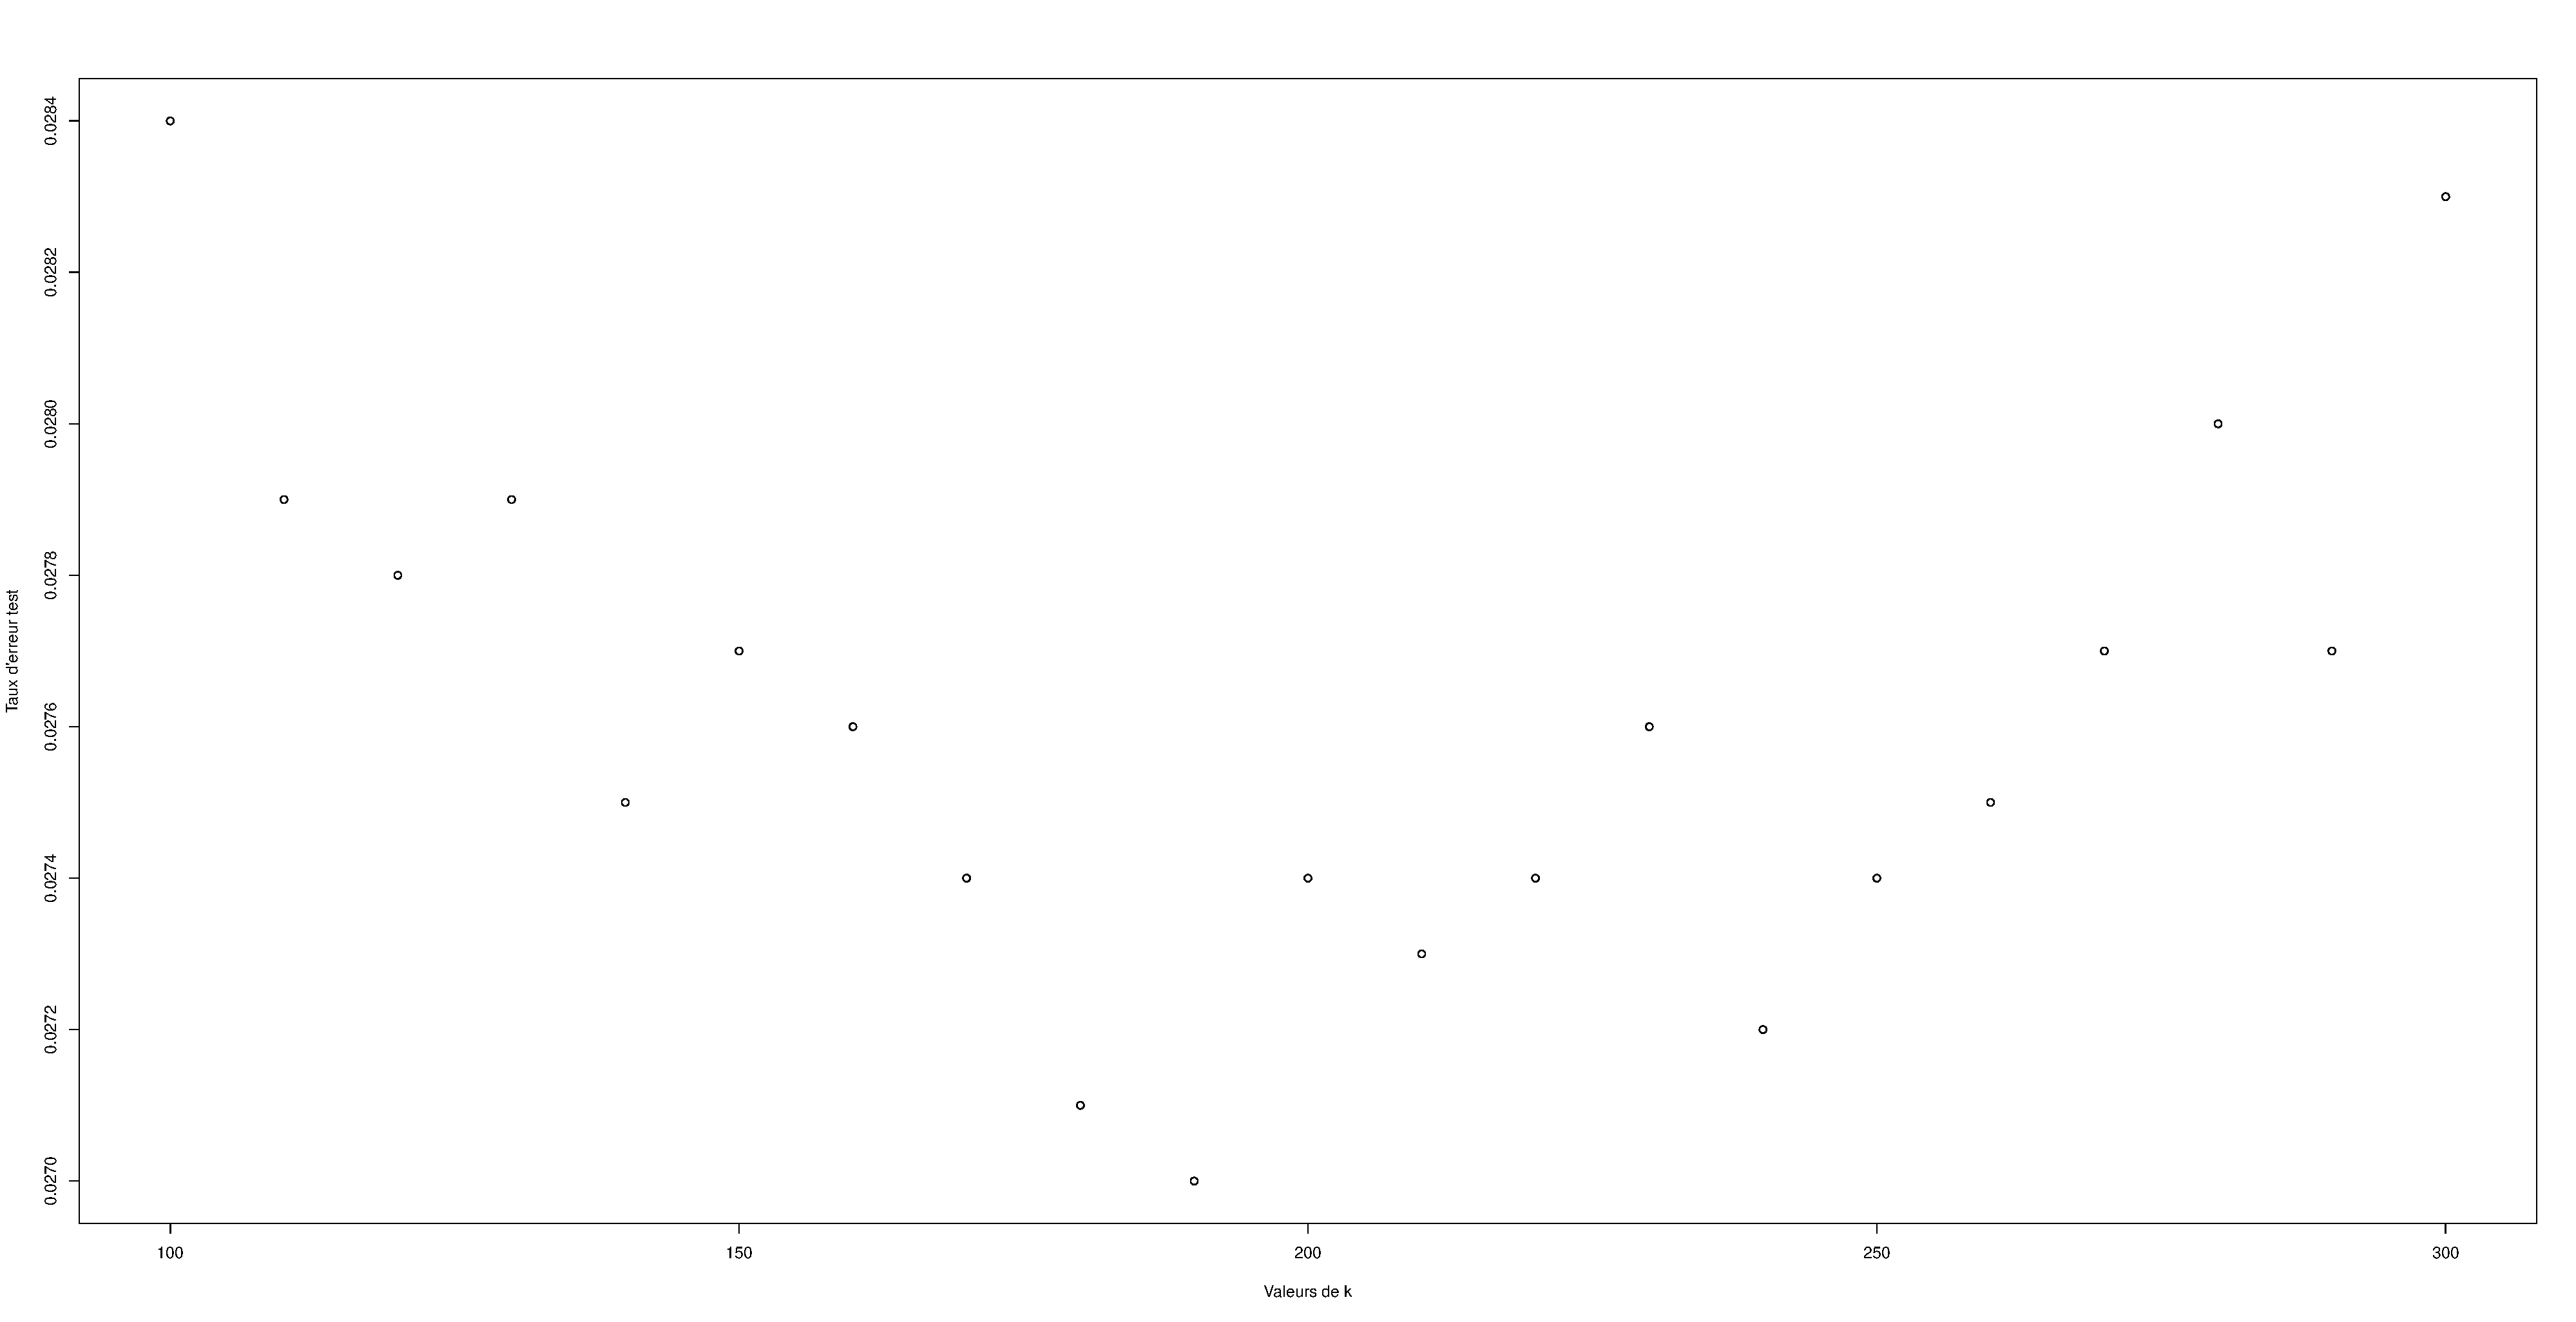
\includegraphics[scale=0.23]{Graphique9.pdf}
\end{center}

\noindent Le taux d'erreur test est minimal pour $k=190$. On illustre le graphique obtenu avec $k=190$.

\begin{verbatim}
> pred_k.min <- knn.reg(train=X,test=axe.x,y=Y,k=k.min)
> plot(X,Y,type="p")
> lines(axe.x$lstat,pred_k.min$pred,col="red")
> title("Regression KNN avec K=k.min qui minimise le taux d'erreur test")
\end{verbatim}

\noindent Et on obtient 
\begin{center}
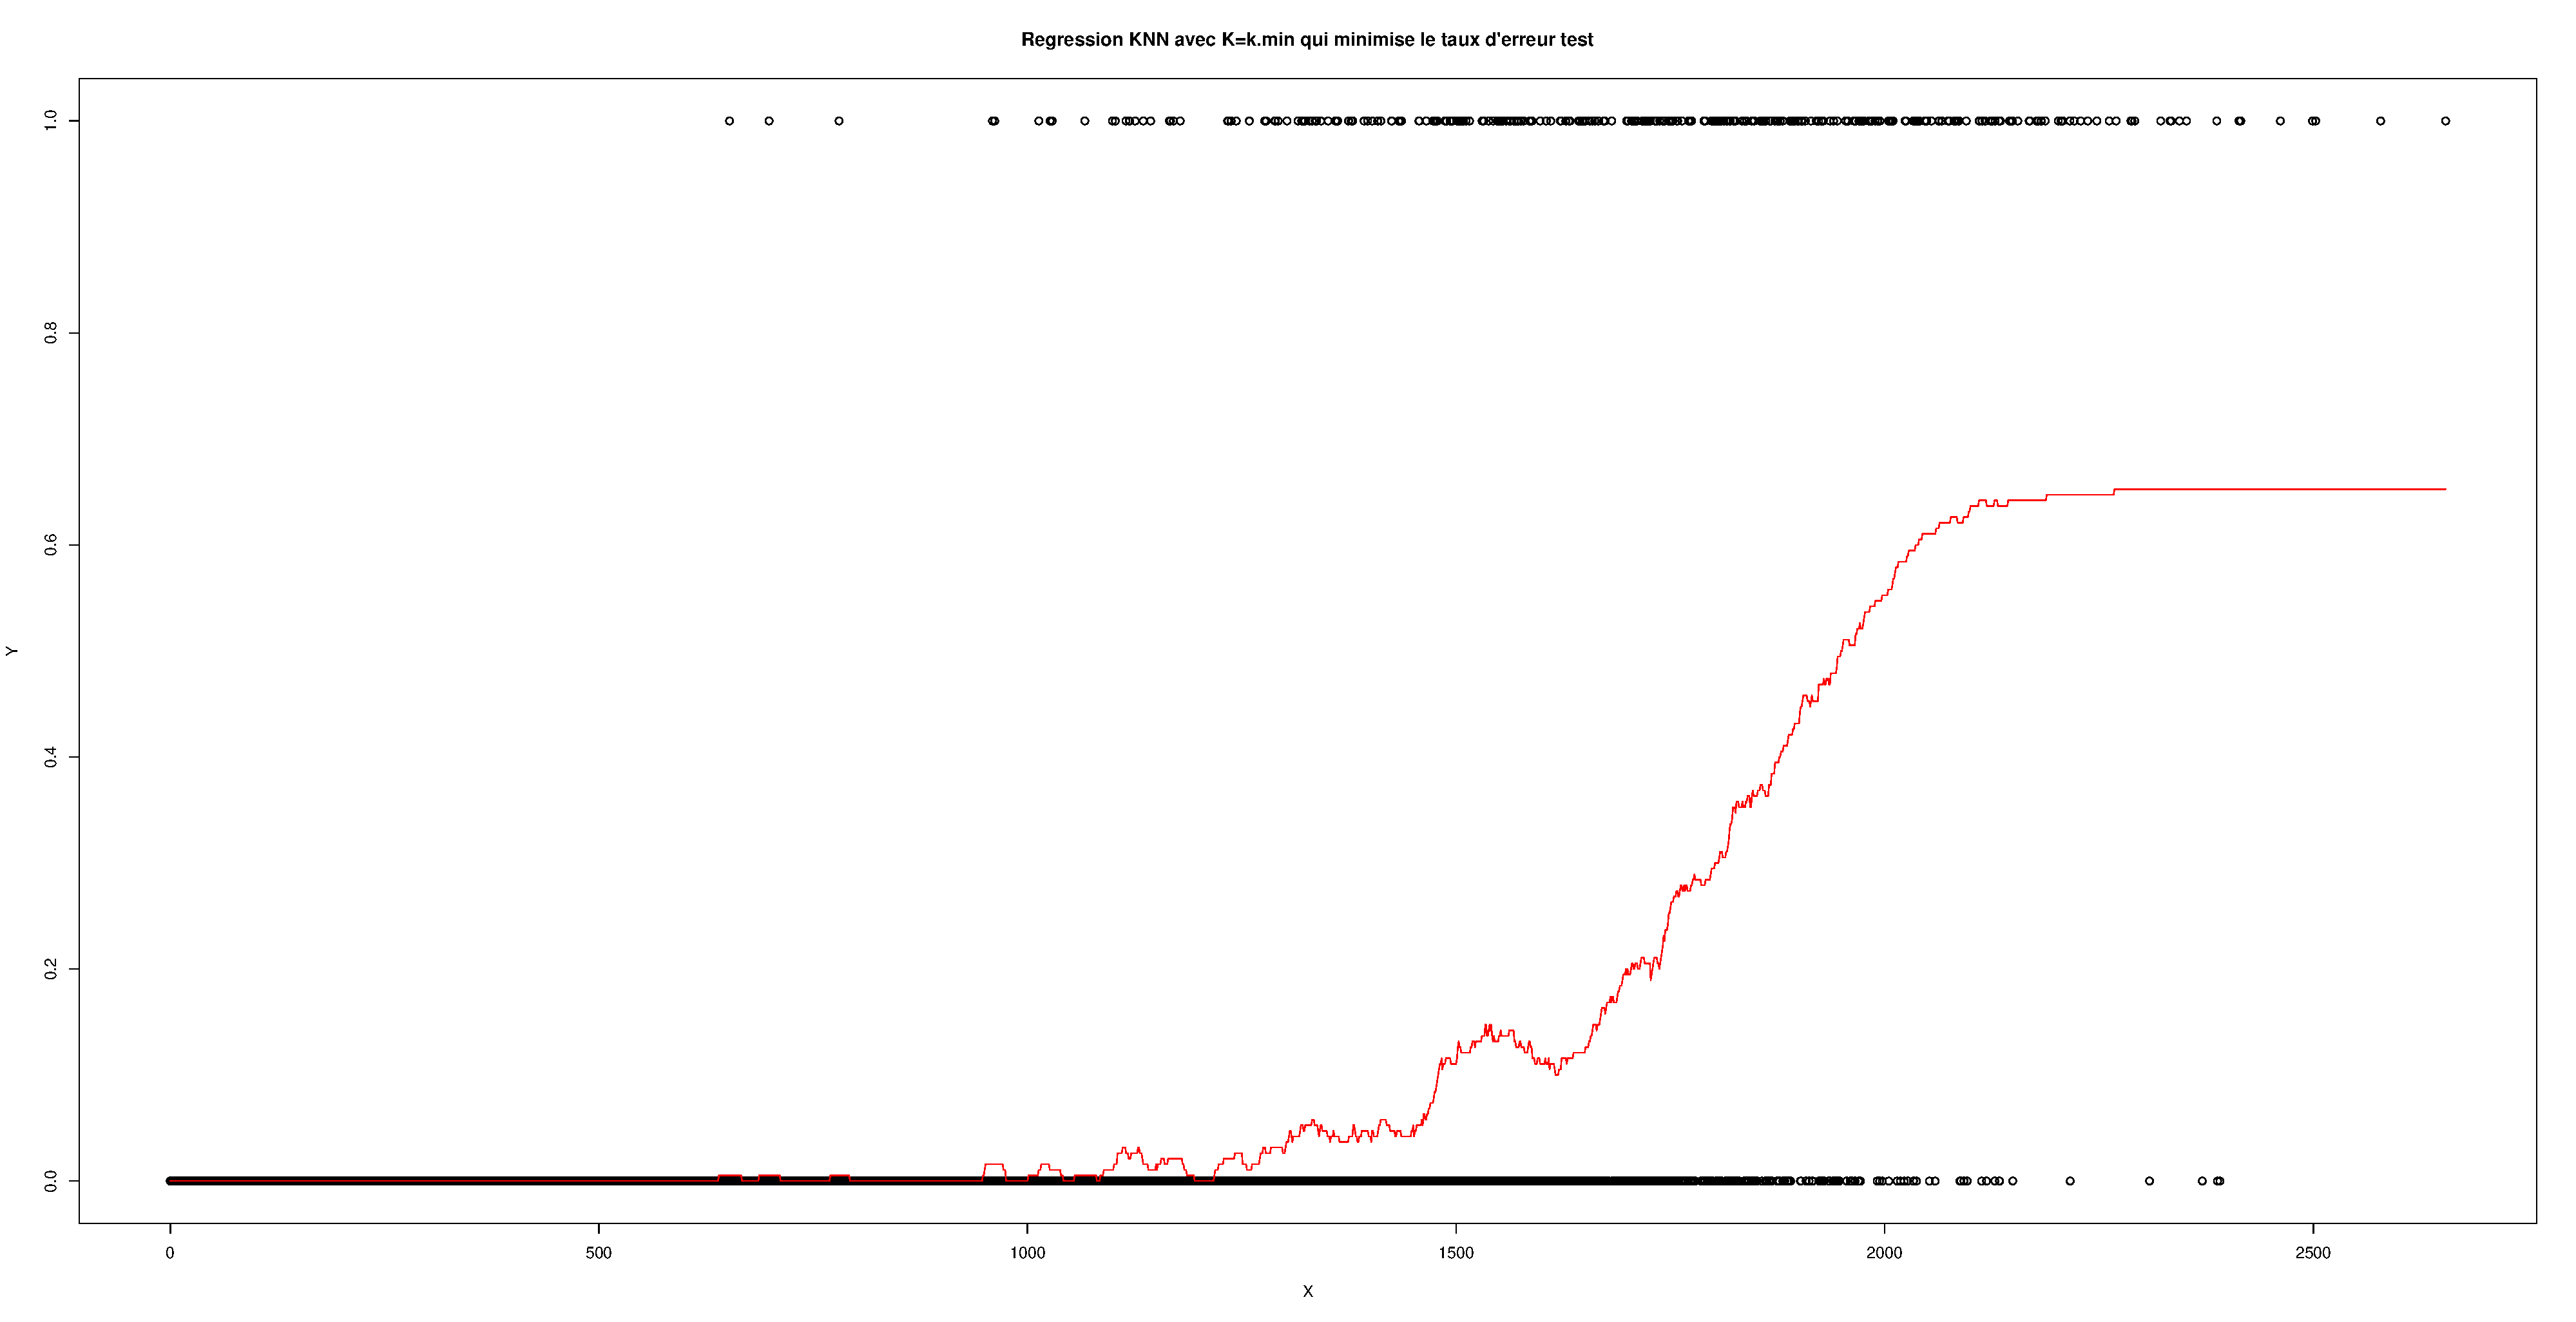
\includegraphics[scale=0.23]{Graphique10.pdf}
\end{center}

\noindent La m\'ethode d\'ecrite ci-haut pour s\'electionner le param\`etre $k$ d\'epend de $u$. Par exemple, avec $u=1/4$, on obtient $k=290$ et avec $u=3/4$, on obtient $k=50$. Le choix de $u$ est arbitraire, m\^eme si $u=1/2$ para\^it un choix naturel. Pour rem\'edier \`a cette probl\'ematique, on peut consid\'erer l'aire sous la courbe ROC comme crit\`ere pour la validation crois\'ee. On choisira alors l'entier $k$ qui maximisera l'aire sous la courbe.

\begin{verbatim}
> library("pROC")#### Installer la librairie pROC
> 
> valeurs.k <- seq(100,300,10)
> res.cv.2 <- NULL
> for (k in valeurs.k)
+ {
+ pred <- knn.reg(train=X,y=Y,k=k)
+ r <- pred$residuals
+ p.hat <- Y - r
+ courbe.roc <- roc(response=Y,predictor=p.hat)
+ res.cv.2 <- c(res.cv.2,courbe.roc$auc)
+ }
> plot(valeurs.k,res.cv.2,xlab="Valeurs de k",
+      ylab="Surface sous la courbe")
> 
> k.max <- valeurs.k[which.max(res.cv.2)]
> k.max
[1] 200
\end{verbatim}

\noindent On s\'electionne $k=200$, ce qui est proche du $k$ s\'electionn\'e par le taux d'erreur test avec $u=1/2$. 

\end{document}

